\pagenumbering{roman}
%\begin{titlepage}
%\begin{center}
%\ \\
%
%\vspace{15mm}
%
%\large
%Univerzita Karlova v Praze\\
%Matematicko-Fyzikální fakulta\\
%
%\vspace{5mm}
%
%{\Large\bf Bakalářská práce}
%
%\vspace{10mm}
%
%%\centerline{\mbox{
\includegraphics[width=60mm]{logo.eps}}}
%
\includegraphics[scale=0.3]{logo.eps} %%% source http://www.mff.cuni.cz/fakulta/symboly/logo.eps
%
%\vspace{15mm}
%%\normalsize
%{\Large Ondřej Plátek}\\ % doplňte vaše jméno
%
%\vspace{5mm}
%{\Large\bf Objektově orientovaná knihovna pro řízení robota e-Puck}
%
%\vspace{20mm}
%\large
%\noindent
%Kabinet software a výuky informatiky \\
%\noindent
% Vedoucí bakalářské práce: RNDr. František Mráz, CSc.\\
% Studijní program: Obecná informatika\\
%\end{center}
%\vspace{20mm}
%\begin{center}
%2011 
%\end{center}
%
%\end{titlepage} % zde končí úvodní strana
%
%\normalsize % nastavení normální velikosti fontu
%\ \vspace{10mm} 
%
%\noindent  Děkuji panu RNDr. Františku Mrázovi, CSc., za~jeho rady
%a nekonečnou podporu při~vedení mé bakalářské práce. Dále jsem vděčný panu Mgr. Pavlu Ježkovi, který
%mi poskytl cenné informace o~technologii .Net. 
%Další díky patří kamarádům Jindřichu Vodrážkovi, Pavlu Menclovi a Adéle Čihákové,
%kteří mě podporovali při~psaní mé bakalářské práce.
%Jidrovi jsem obzvlášť vděčný za jeho odvahu, když použil nedokončenou verzi {\it Elib} knihovny pro svůj projekt. 
%V~projektu úspěšně implementoval Breitenbergovo chování pro robota e-Puck.
%V~neposlední řadě bych rád poděkoval rodičům za~veškerou jejich péči a podporu.
%
%\vspace{\fill} % nastavuje dynamické umístění následujícího textu do spodní části stránky
%\noindent 
%Prohlašuji, že jsem tuto bakalářskou práci vypracoval(a) samostatně a výhradně
%s~použitím citovaných pramenů, literatury a dalších odborných zdrojů.
%
%\medskip\noindent
%Beru na~vědomí, že se na~moji práci vztahují práva a povinnosti vyplývající
%ze~zákona č. 121/2000 Sb., autorského zákona v~platném znění, zejména skutečnost,
%že Univerzita Karlova v~Praze má právo na~uzavření licenční smlouvy o~užití této
%práce jako školního díla podle §60~odst. 1~autorského zákona.
%
%\bigskip
%\noindent V Praze dne 5. dubna 2011 \hspace{\fill}Ondřej Plátek\\ 
%
%%%%   Výtisk pak na tomto místě nezapomente PODEPSAT!

\begin{titlepage}
\begin{center}
\ \\

\vspace{15mm}

\large
Charles University in Prague\\
Faculty of Mathematics and Physics\\

\vspace{5mm}

{\Large\bf BACHELOR THESIS}

\vspace{10mm}


\includegraphics[scale=0.3]{logo.eps} %%% source http://www.mff.cuni.cz/fakulta/symboly/logo.eps

\vspace{15mm}
%\normalsize
{\Large Ondřej Plátek}\\ 

\vspace{5mm}
{\Large\bf Object Oriented Library for Controlling an e-Puck Robot}

\vspace{20mm}
\large
\noindent
Department of Software and Computer Science Education

\noindent
 Supervisor: RNDr. František Mráz, CSc.\\
 Study branch: General Informatics\\
\end{center}
\vspace{20mm}
\begin{center}
2011
\end{center}

\end{titlepage} % zde koncí úvodní strana

\normalsize % nastavení normální velikosti fontu
\vspace{10mm} 

\noindent I would like to thank my supervisor, RNDr. František Mráz, CSc., for his
advice and endless support. I am grateful to Mgr. Pavel Ježek, who gave me 
valuable informations about .Net technology. 
My sincere gratitude belong to my friends Jindřich Vodrážka, Pavel Mencl and Adéla Čiháková,
who has supported me during writing of my bachelor thesis.
Jidra has the courage to use the~unfinished {\it Elib} library developed in this thesis in his project and
he successfully implemented a Breitenberg behaviour for e-Puck robot.
Last but not least I would like to give thanks to my patient parents for all their efforts.


\vspace{\fill} % nastavuje dynamické umístění následujícího textu do spodní části stránky
\noindent
I declare that I wrote my bachelor thesis independently and exclusively with~the~use of the cited sources. I agree~with lending and publishing this thesis.

%\medskip\noindent
%I acknowledge that my thesis is a~subject to the stipulations of rights and obligations of the Act No. 121/2000 Coll., Copyright Act as valid, especially the~fact that Charles University in~Prague has a right to conclude a~licence agreement on~the use of the~school work as per sect. 60, paragraph 1 of~the~Copyright Act.

\medskip\noindent
I declare that I carried out this bachelor thesis independently, and only with the cited
sources, literature and other professional sources.

I understand that my work relates to the rights and obligations under the Act No.
121/2000 Coll., the Copyright Act, as amended, in particular the fact that the Charles
University in Prague has the right to conclude a license agreement on the use of this
work as a school work pursuant to Section 60 paragraph 1 of the Copyright Act.

\noindent Prague, April 5, 2011 \hspace{\fill}Ondřej Plátek 

%%%   Výtisk pak na tomto míst+ nezapomente PODEPSAT!
%%%                                         *********

%\begin{figure}[htp] \centering{
%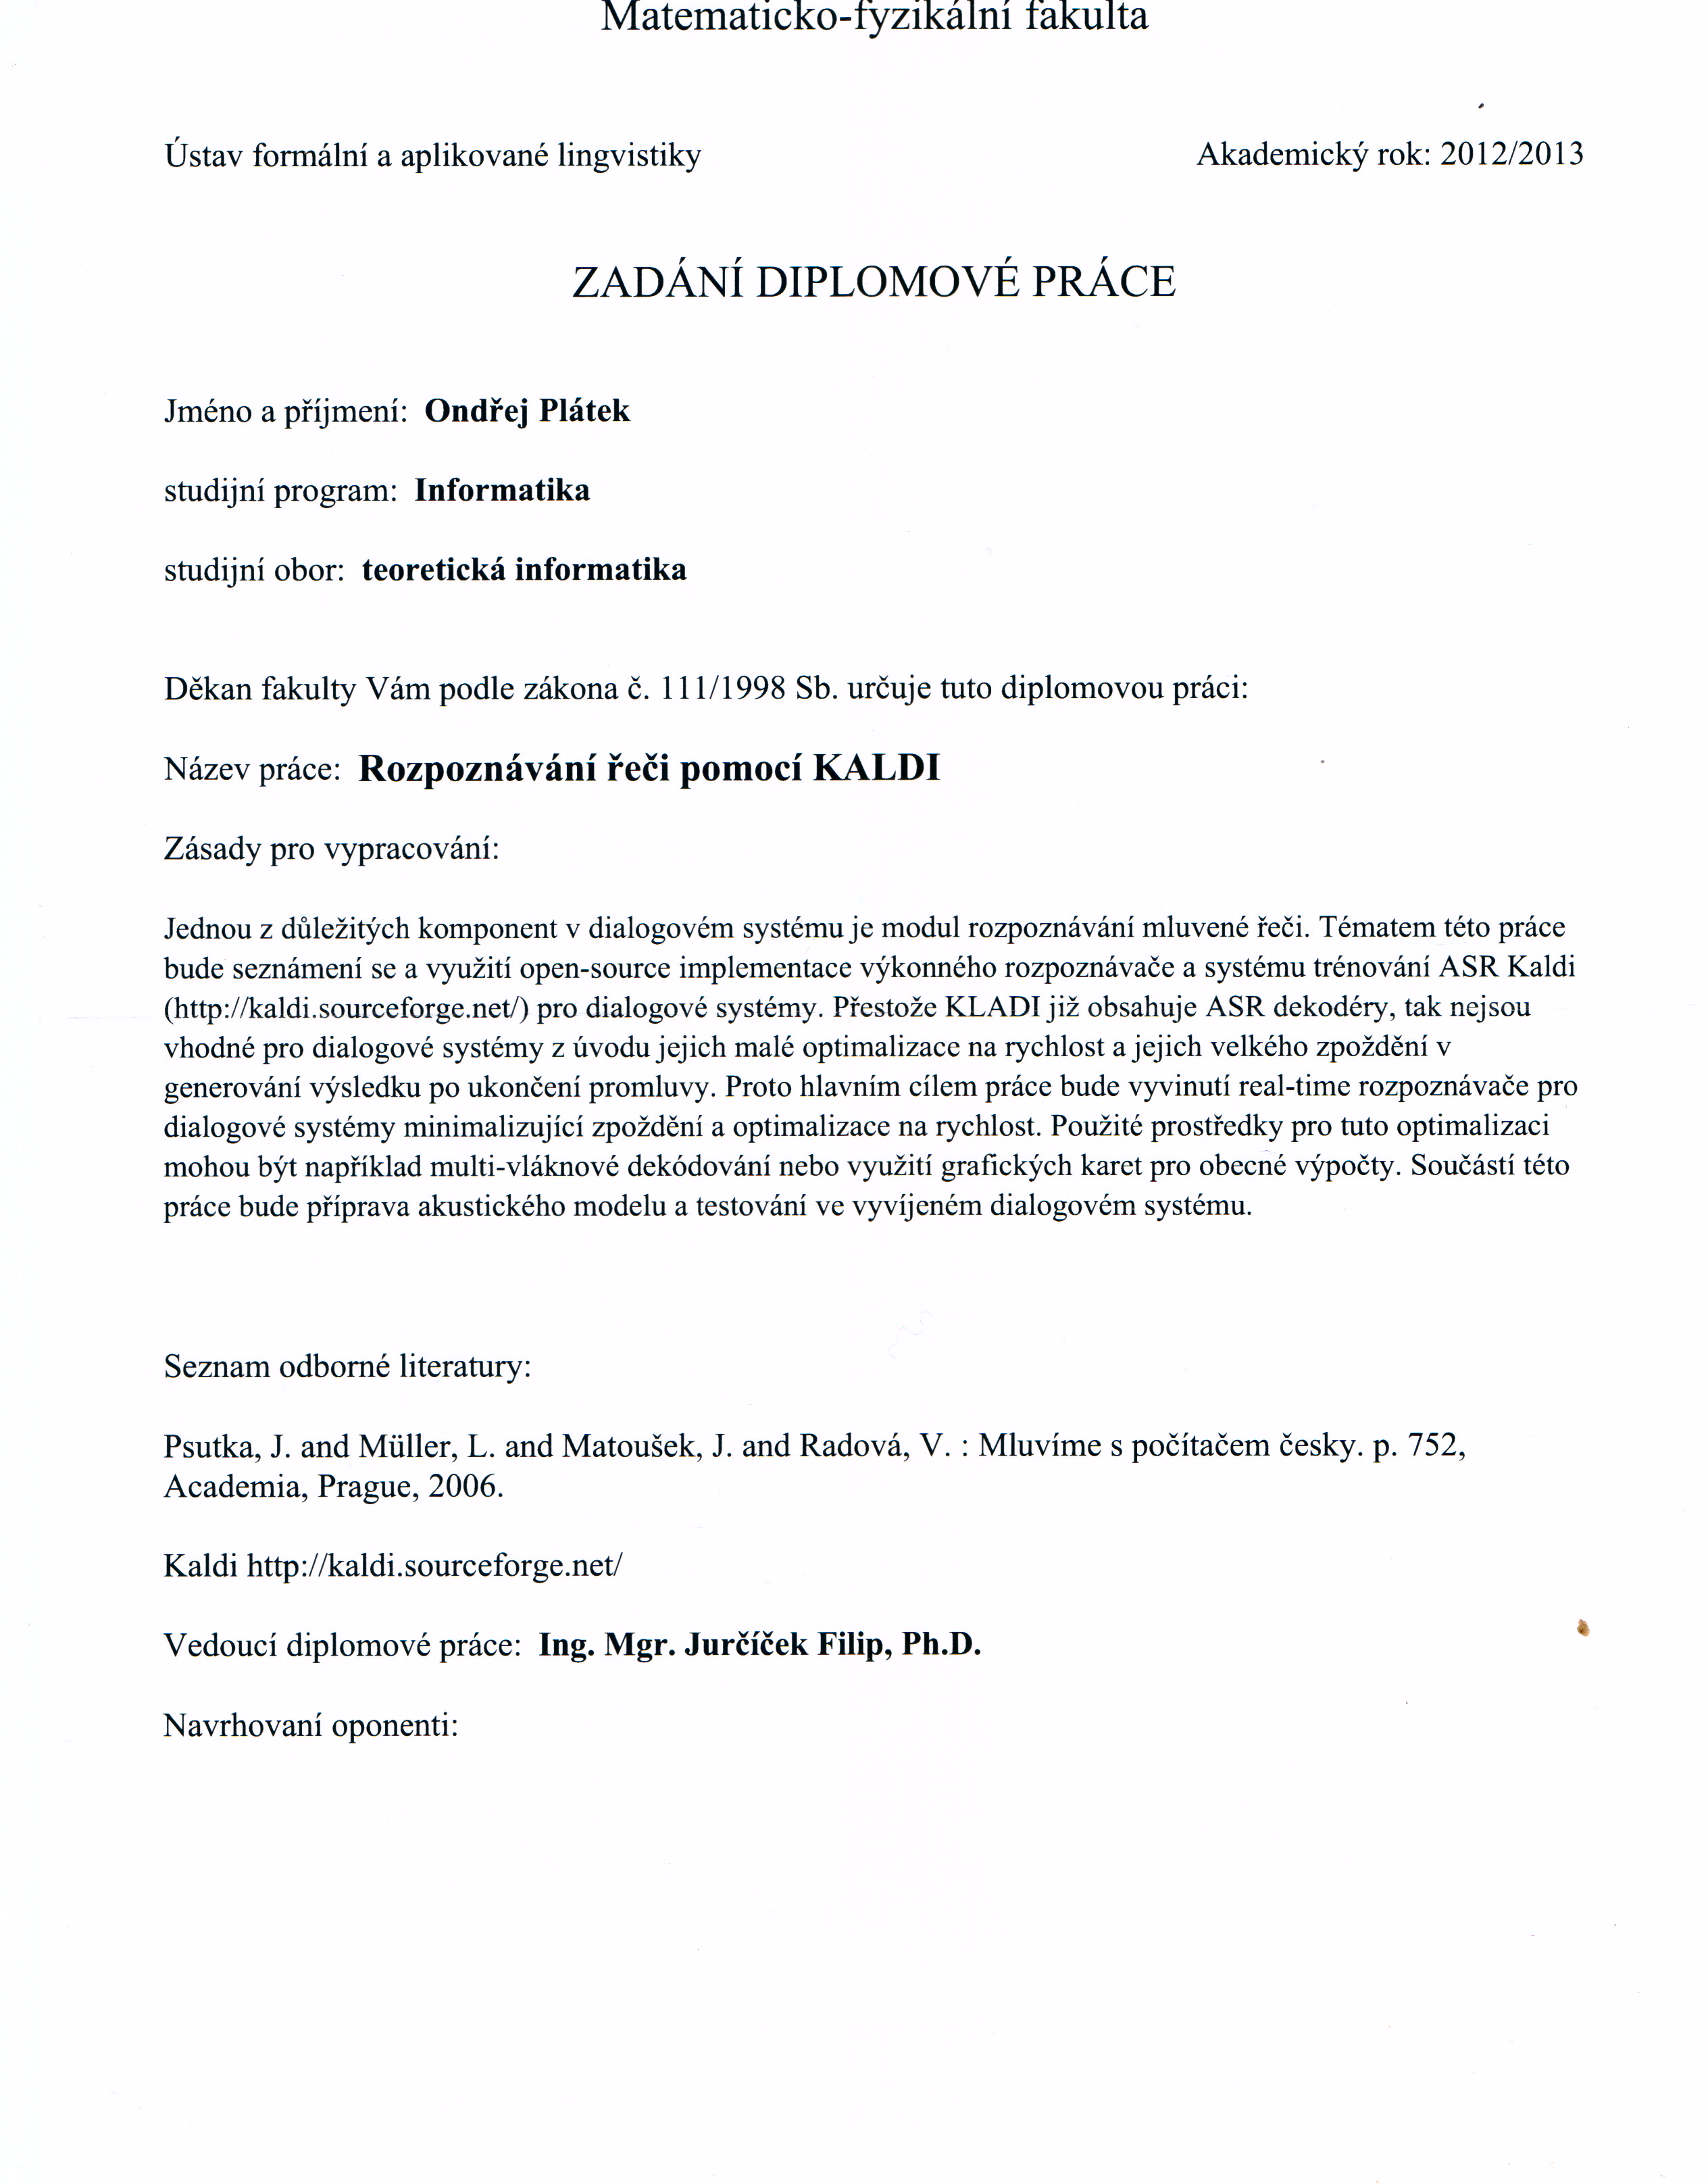
\includegraphics[scale=0.82]{zadani1}}
%\end{figure}  
%
%\newpage
%\begin{figure}[htp] \centering{
%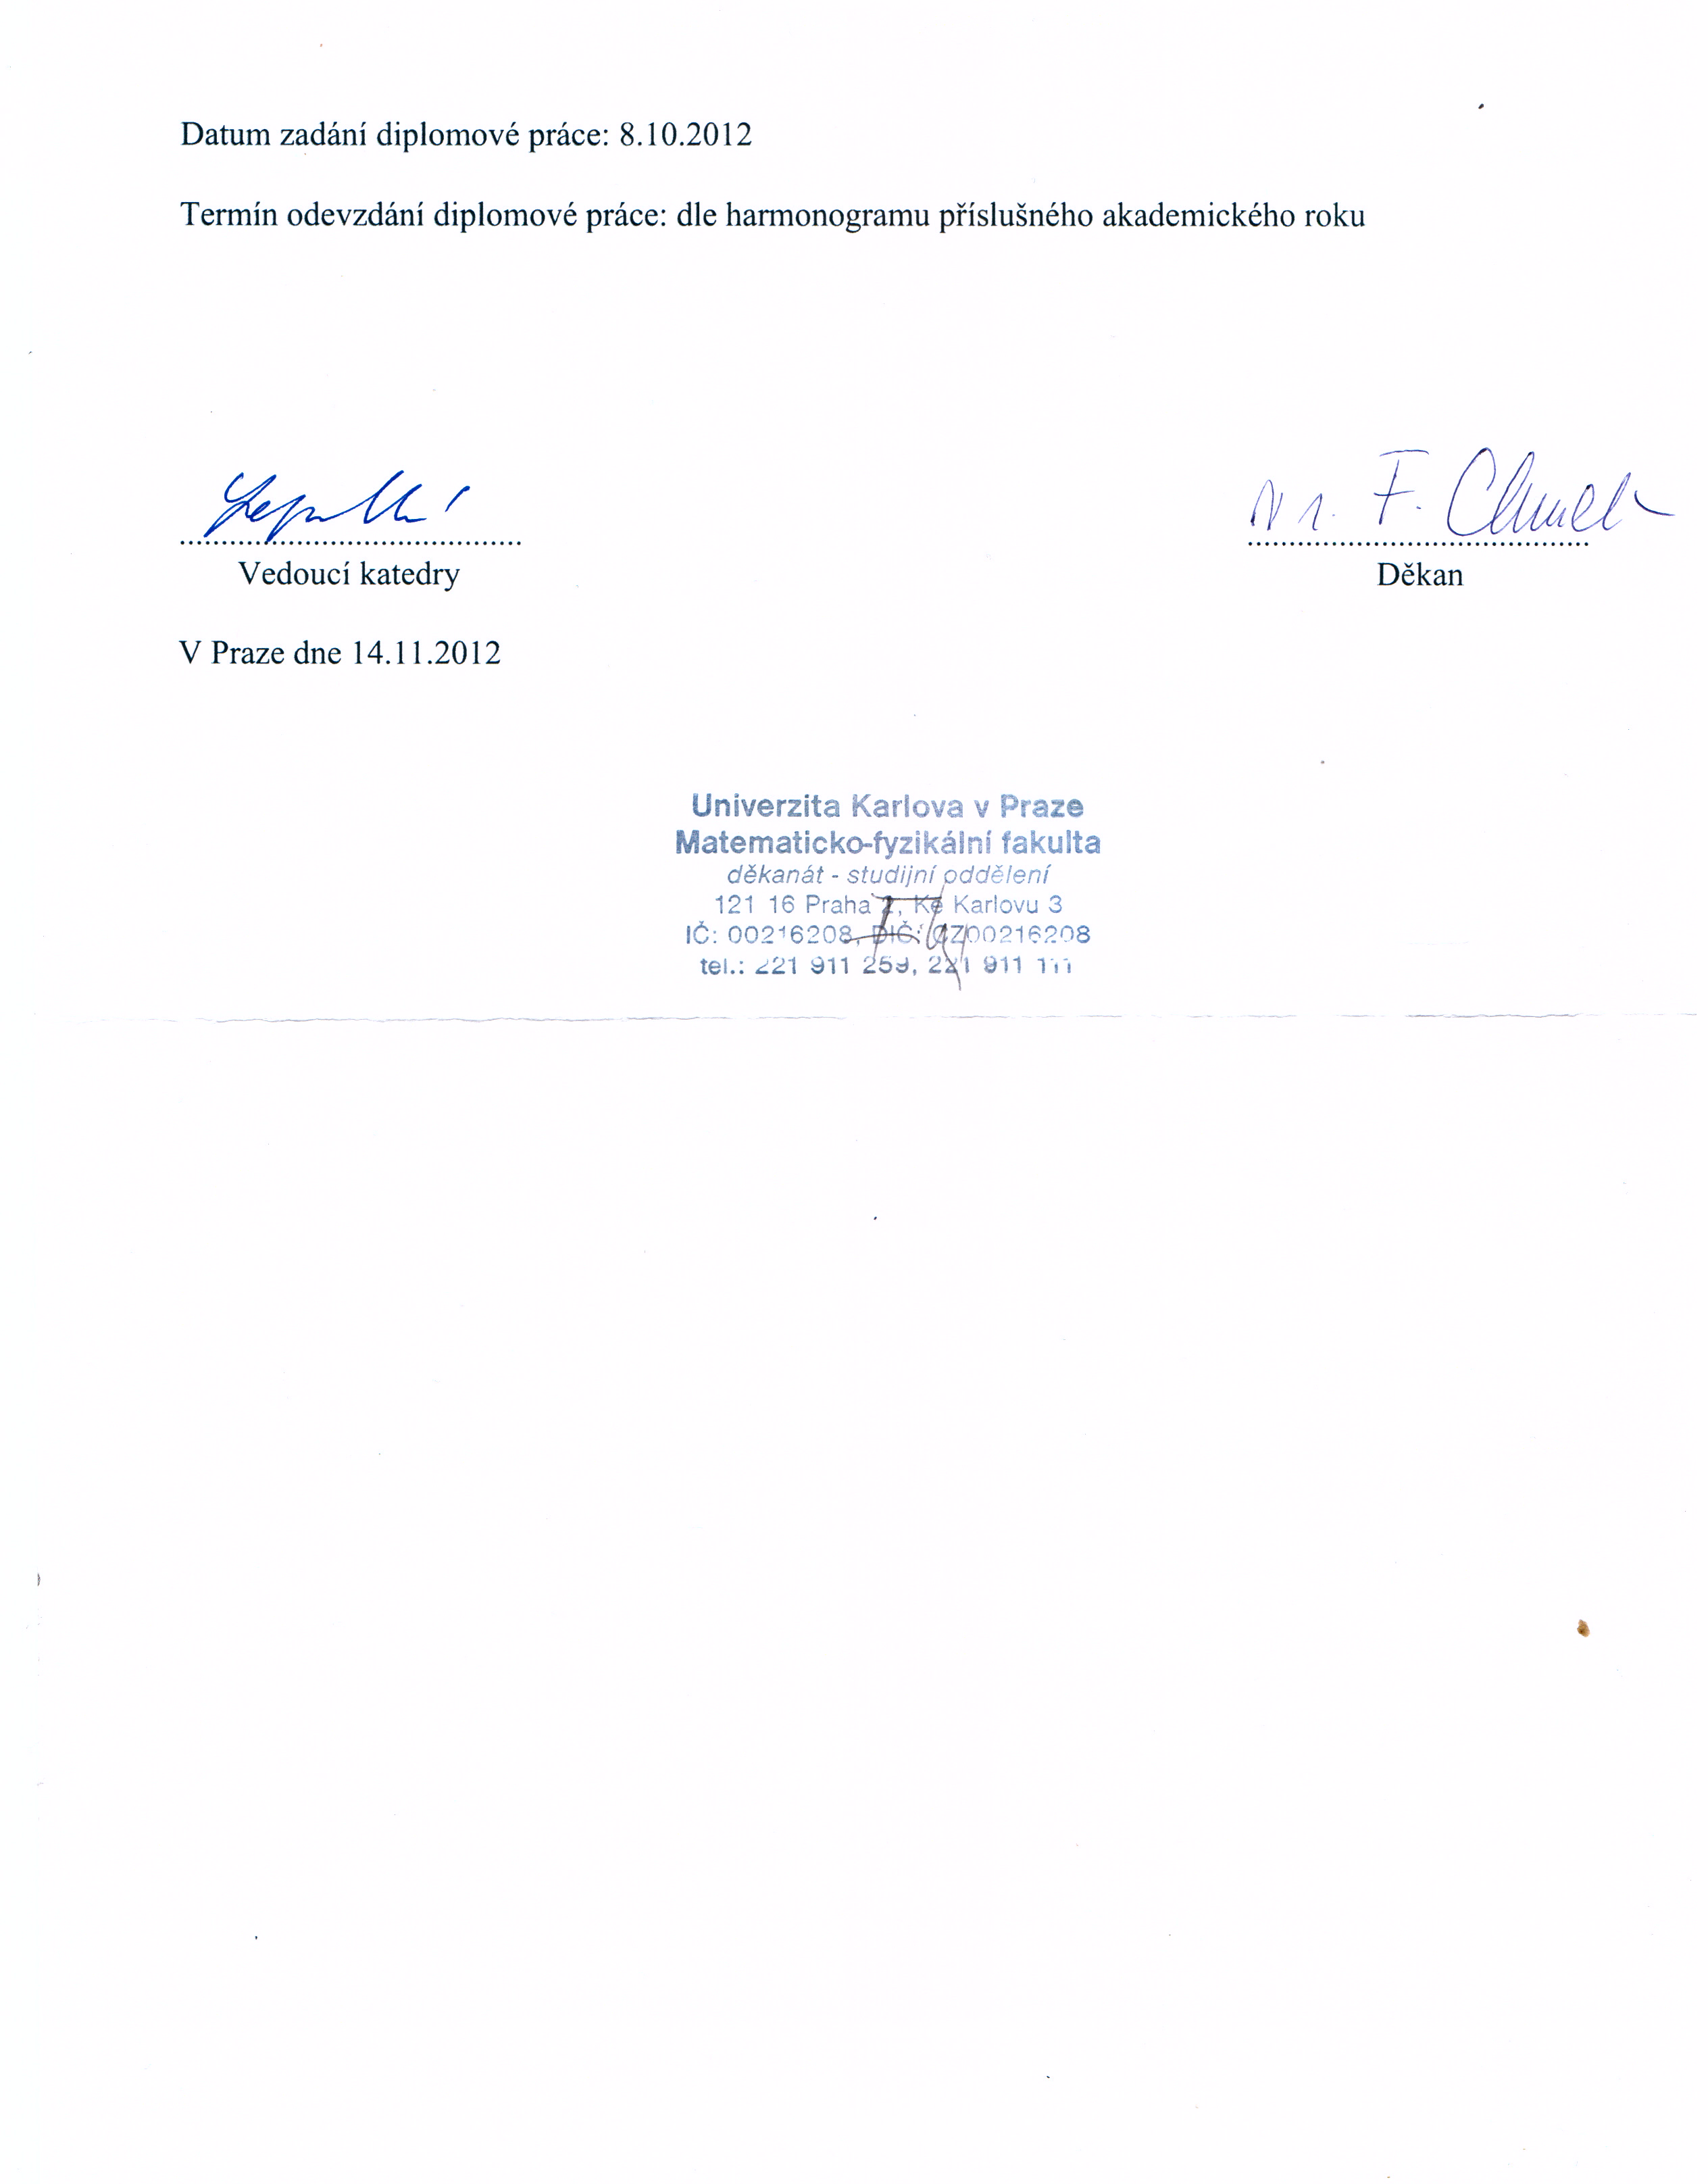
\includegraphics[scale=0.82]{zadani2}}
%\end{figure}  

\newpage

%%% Následuje strana s abstrakty. Doplnte vlastní údaje.
\vbox to 0.5\vsize{
\setlength\parindent{0mm}
\setlength\parskip{5mm}
Název práce: Objektově orientovaná knihovna pro řízení robota e-Puck\\
Autor: Ondřej Plátek\\
Katedra: Kabinet software a výuky informatiky\\
Vedoucí bakalářské práce: RNDr. František Mráz, CSc.\\
e-mail vedoucího: Frantisek.Mraz@mff.cuni.cz\\

\noindent Abstrakt: E-Puck je  výukový robot s diferenciálním pohonem dvou kol, který je adekvátně vybaven senzory.
Výsledkem práce je objektová $C\#$ knihovna {\it Elib}, která umožňuje
ovládat robota e-Puck z hostitelského počítače přes Bluetooth rozhraní.
Vzorové příklady v konsolové aplikaci {\it TestElib} ukazují použití knihovny {\it Elib} v~programech pro ovládání robota e-Puck.
Taktéž je přiložena sada nástrojů umožňující efektivnější ladění programů používající {\it Elib} library.

\noindent Klíčová slova: robot, e-Puck, asynchronní, $C\#$, knihovna

\vspace{10mm}

\noindent
Title: Object Oriented Library for Controlling an e-Puck Robot\\
Author: Ondřej Plátek\\
Department: Kabinet software a výuky informatiky \\
Supervisor: RNDr. František Mráz, CSc.\\
Supervisor's e-mail address: Frantisek.Mraz@mff.cuni.cz\\

\noindent Abstract: E-Puck is an educational robot with differential drive and 
it is sufficiently equipped with sensors. The result of present thesis is the $C\#$ object oriented {\it Elib} library, 
which allows to control an e-Puck robot from a host computer over the Bluetooth wireless technology. 
The model examples in the {\it TestElib} console application presents 
the~usage of the {\it Elib} library in~program for the e-Puck robot. 
Moreover, it offers a comfortable system of help and documentation.
Enclosed sets of tools allows more effective debugging of programs, 
which use the {\it Elib} library.

\noindent Keywords: robot, remote control, e-Puck, asynchronous, $C\#$, library

\vss}

\newpage

\openright
\pagestyle{plain}
\pagenumbering{arabic}
\setcounter{page}{1}
\tableofcontents


